\section{Votación \onchain e incentivos}

Nebulas se dedica a la gobernanza \onchain y su compromiso es el de utilizar la tecnología \blockchain para proporcionar un entorno más abierto y colaborativo.

\subsection{Proceso de gobernanza \onchain}
\label{governance}

El proceso general de la gobernanza \onchain en Nebulas es como se describe a continuación:~\ref{fig:on-chain-governance}:

\begin{figure}
	\centering
	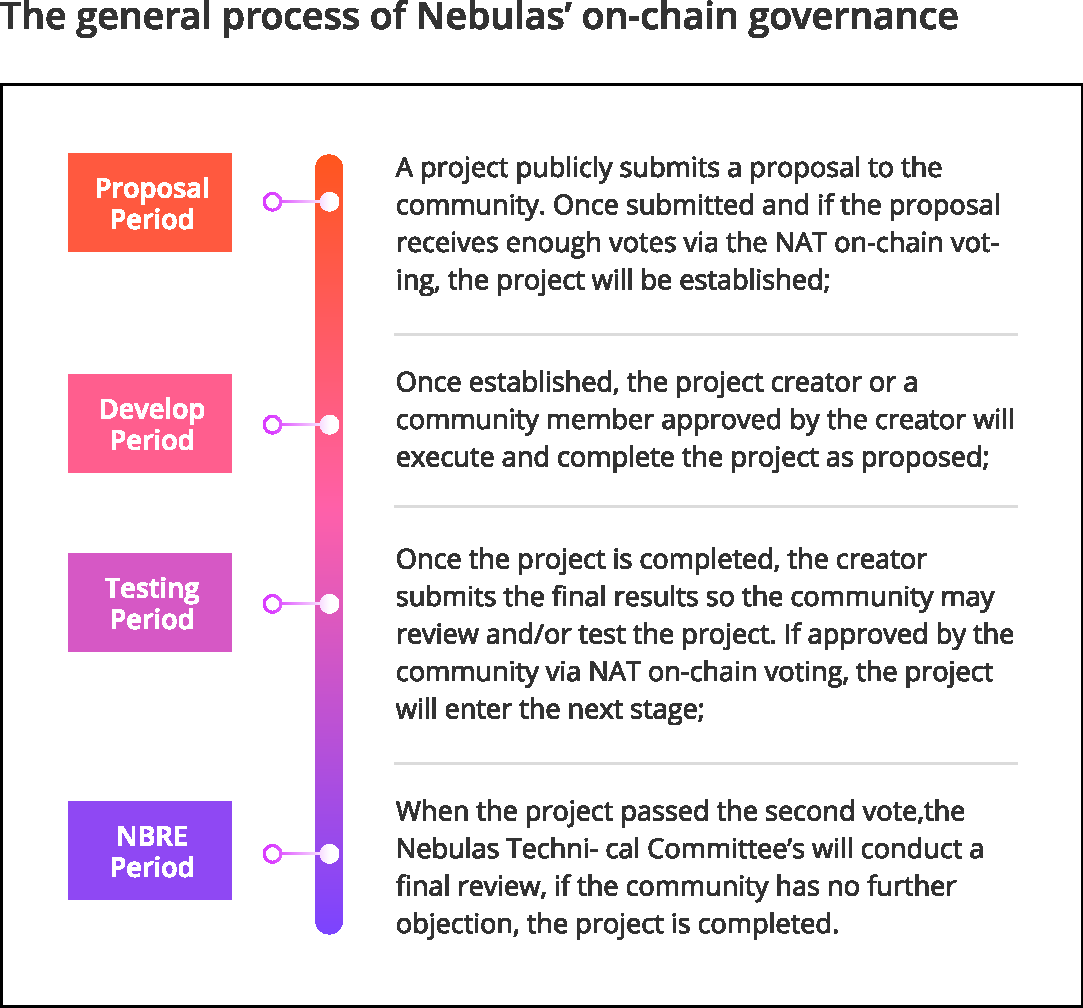
\includegraphics[width=1\textwidth]{../common/en/on-chain-governance.pdf}
	\caption{Proceso de gobernanza \onchain de Nebulas \label{fig:on-chain-governance}}
\end{figure}

\begin{enumerate}
	\item \textbf{Periodo de propuesta}: Se presenta públicamente una propuesta a la comunidad. Una vez presentada, y si la propuesta recibe suficientes votos a través de la votación NAT \onchain, se aprobará la ejecución del proyecto;
	\item \textbf{Periodo de desarrollo}: Una vez aprobado, el creador del proyecto —o el miembro de la comunidad aprobado por el creador— se encargará de ejecutar y completar el proyecto tal como se propuso;
	\item \textbf{Periodo de pruebas}: Una vez finalizado el proyecto, el creador enviará el resultado final para que la comunidad lo someta a revisión. Si la comunidad lo aprueba por medio del voto NAT \onchain, el proyecto pasará a la fase final;
	\item \textbf{Periodo \textit{NBRE}}: Cuando el proyecto pasa la segunda votación (revisión de la comunidad), el Comité Técnico de Nebulas realizará una revisión final. Si la comunidad no plantea ninguna objeción, el proyecto se marcará como completo.
\end{enumerate}

La gobernanza \onchain se basa en dos propiedades:

\begin{enumerate}
	\item La votación utiliza el token de gobernanza NAT y sus algoritmos subyacentes.
	\item El proceso de votación es bizantino, mediante tecnología \blockchain.
\end{enumerate}

Este Libro Naranja cubre principalmente los aspectos de la gobernanza \onchain.

\subsection{Principios básicos de votación}

El ecosistema de Nebulas integra las votaciones en su red principal. Cada voto emitido por los miembros de la comunidad es transparente y visible para todos. Dentro de Nebulas, la votación utiliza los siguientes principios básicos:

\begin{enumerate}
	\item La unidad básica de votación es una dirección \textit{mainnet} de Nebulas.
	\item El peso de los votos se referirá a la valuación de la dirección, dada por \nr.
	\item Las contribuciones positivas de los usuarios al sistema serán recompensadas con más derechos de voto. Creemos que la votación es una contribución positiva al ecosistema de Nebulas y que los usuarios deben estar motivados a recibir más derechos de voto.
\end{enumerate}

\subsection{Método de votación}

La votación será operada a través de un contrato inteligente en la red principal del \blockchain de Nebulas. Cada dirección podrá elegir entre tres opciones:

\begin{itemize}
	\item A favor
	\item En contra
	\item Abstención.
\end{itemize}

En forma adicional, los usuarios podrán decidir simplemente no ejercer su derecho a voto.

\subsection{El único medio utilizado para la votación: NAT}

\label{nat}

\subsubsection{Descripción general}

\begin{itemize}
	\item \textbf{Nombre}: Nebulas Autonomous Token
	\item \textbf{Símbolo bursátil (\textit{ticker})}: NAT
	\item \textbf{Estándar}: token NRC20
\end{itemize}

El Token Autónomo de Nebulas (\textit{Nebulas Autonomous Token, o NAT}) es un activo derivado de Nebulas Rank que se materializará en la forma de un token NRC-20, y que servirá como el único medio de voto dentro de la gobernanza del ecosistema Nebulas.

\begin{center}
	\fboxsep24pt
	\colorbox{yellow!30}{
	\begin{minipage}[c]{.8\textwidth}
		\paragraph{¿Qué es Nebulas Rank?}
		Nebulas Rank (NR) es el primer mecanismo nativo \onchain de medición de valor multidimensional de los datos \blockchain.

		Dentro de la economía de Nebulas, la unidad básica de gobernanza es una \emph{dirección}
		(\ref{rights}). Nebulas Rank cuantifica la contribución de cada
		\emph{individuo} a la acumulación económica por medio de la expresión matemática de la contribución de cada dirección. Nebulas Rank se divide en \emph{Core
		Nebulas Rank} y \emph{Extended Nebulas Rank}. Core Nebulas Rank refleja principalmente dos factores: el valor medio de una cuenta dentro de un período de tiempo determinado, y el grado de utilización de activos de esa cuenta durante un periodo de tiempo.

		A nivel macro, la relación entre el número de divisas, el valor del dinero, la tasa de circulación y la productividad dentro del \blockchain se puede describir con la ecuación clásica de la cantidad de dinero. El valor NR de la red entera refleja la liquidez total del ecosistema Nebulas, como así también su actividad.

		\paragraph{NAT y NR}

		La publicación de NAT se refiere principalmente a \emph{Core Nebulas Rank}, que muestra el rendimiento de los activos. En cada emisión semanal de NAT se revisará el valor NR con referencia al promedio y grado de utilización de los activos. Para más información en el sistema de valuación Nebulas Rank, sírvase consultar el \yellowp, publicado por el Instituto de Investigaciones de Nebulas en junio de 2018.

		\paragraph{¿Cómo se verifica mi valor Nebulas Rank?}

		Nebulas Rank, a través de Nebulas NOVA~\cite{nova} recibió su primera actualización el 6 de mayo de 2019. Esta actualización hizo uso del \textit{Nebulas Blockchain Runtime Environment (NBRE)} para lograr una actualización instantánea y autónoma. El algoritmo Nebulas Rank es de código abierto y se puede consultar en línea~\cite{CheckNR}.

	\end{minipage}}
\end{center}

\subsubsection{Casos de uso para el \textit{Nebulas Autonomous Token} (NAT)}

NAT is the only voting medium within Nebulas. Community members can vote on-chain via the NAT token to decide the direction of the Nebulas ecosystem. These decisions include but are not limited to: the election of Nebulas Council members, adjustments to the Nebulas Protocol Representation(NPR) via the Nebulas Blockchain Executable Environment (NBRE), establish, vote and review community proposals.

\subsubsection{Release}

The distribution method of NAT is similar to that of Bitcoin with the premise that there is an upper limit on the total supply and the distributed supply is decremented weekly.

The supply upper limit of NAT tokens is related to the Nebulas Rank score of
the entire Nebulas mainnet. The release amount is decremented weekly and the
attenuation coefficient is $\lambda$. The initial value of $\lambda$ is 0.997; this means that by week 180, the circulation is decremented to 58\% of the first week.

The initial circulation of NAT is based on the status of Nebulas NOVA mainnet after the completion of it's first voting upgrade on May 6th, 2019. Based on the current Nebulas Rank of the entire network and initial parameters, the upper limit of the total amount of NAT to ever exist will be 100 billion.

\subsubsection{Managing NAT}

Users can manage their NAT via NAS nano Pro~\cite{NASnano} and other wallets that support Nebulas NRC20~\cite{wallets} tokens. Users can view NAT transactions and circulation on blockchain explorers~\cite{explorer} that support the Nebulas mainnet.

\subsection{Obtaining NAT}

All users who control Nebulas mainnet addresses (with the exception of black listed address) have the opportunity to receive NAT. Address holders can obtain NAT via three ways: improve the Nebulas Rank score of the address, participate in Nebulas on-chain voting and by pleading NAS.

\paragraph{NAT blacklisted addresses}

During the NAT distribution process, any address that conflicts with any of
Nebulas \emph{address} basic rights (~\ref{rights}) will be classified as a blacklisted address.

Blacklist addresses can only obtain partial NAT based on their rights. For example, the address of a centralized exchange is classified as a blacklist address. According to the first basic right of Nebulas address owners, the address has the right to own and operate their assets on Nebulas; in return, the exchange address can obtain NAT under the same conditions according to the Nebulas Rank of the address. However, the collected property (NAT) of the exchange should be distributed to the corresponding exchange user. According to the second and third basic rights Nebulas address ownership, the exchanges collection address does not have the right to initiate a proposal or to participate in proposal vote before the exchange proves that the collection address fully represents the corresponding custody asset user proposal and voting willingness. Therefore, blacklisted addresses cannot obtain a NAT incentive by participating in the voting.

\subsubsection{Receive NAT by improving the Nebulas Rank score of an address}

NAT tokens will be distributed to Nebulas mainnet address which have a positive NR score on a weekly basis. The number of NAT tokens distributed will be based on the weekly Nebulas Rank of the address and the Nebulas Rank of the entire mainnet.

The number of distributed tokens will be decremented weekly. The attenuation coefficient is $\lambda$. Initially $\lambda$ = 0.997.

In the $i$th week, the ratio is:

\begin{align}
1\,\text{NR}=z(x_{ne},x_{e},\mu)\times\lambda^{i}\,\text{NAT}
\end{align}

Above Formula breakdown:

\begin{itemize}
	\item $\lambda$: attenuation coefficient.
	\item $\mu$: incentive parameters for voting behavior.
	\item $x_{ne}$: the sum of the NR score of non-exchange address on the entire mainnet.
	\item $x_{e}$: NR sum of the entire mainnet.
	\item $z(x_{ne},x_{e},\mu)$: function with $x_{ne}$, $x_{e}$ and $\mu$ as variables, Nebulas Rank and NAT redemption proportion.
\end{itemize}

\subsubsection{Pledging NAS to receive NAT}

Starting May 6, 2019, users of Nebulas mainnet can choose to obtain NAT by
\emph{pledging} Nebulas native coin NAS via a smart contract.

Users of the Pledge NAS smart contract will receive NAT beginning the second week after pledging begins (May 13, 2019). If users cancel their pledge, NAT distribution will cease.

The number of distributed tokens per week will be decremented. The attenuation coefficient is $\lambda$. Initially $\lambda$ = 0.997.

The ratio of pledge NAS to NAT during the $i$th week:

\begin{align}
x\,\text{NAS} \rightarrow \alpha \times z(x_{ne},x_{e},\mu)\times g(x) \times
  \lambda^{i}\,\text{NAT}
\end{align}

Above Formula breakdown:

\begin{itemize}
	\item $x$: the number of pledged NAS.
	\item $\alpha$: the pledge coefficient, $\alpha$=5 in the initial state.
	\item $z(x_{ne},x_{e},\mu)$: function with $x_{ne}$, $x_{e}$, and $\mu$ as variables, the exchange ratio of NR and NAT.
	\item $g(x)$: A function associated with $x$ that simulates the Nebulas Rank obtained by the NAS with a $x$ value on the Nebulas mainnet.
\end{itemize}

\paragraph{How to start pledging?}
To begin a pledge, users will need to send a transaction to the voting smart contract via their Nebulas wallet such as NAS nano Pro or other wallets that support the Nebulas mainnet. In return, the pledged NAS will be locked in the smart contract until the pledge is canceled by the user.

In order to guarantee the acquisition of NAT, the user must send their NAS to the Pledge smart contract address via a user controlled address which they hold the private key to. Users must not send NAS to the pledge smart contract directly from an exchange or address you do not fully control.

\paragraph{How to cancel pledging?}

If a user wants to cancel their pledge and unlock their NAS, NAS nano Pro or other supported wallets can interact with the smart contract to cancel the pledge. After canceling, the pledged NAS will be unlocked and will become available to the user.

\subsubsection{Receive NAT through Nebulas on-chain voting}

The NAT will be conducted at the beginning of every week on the Nebulas
mainnet. Once addresses obtain NAT, they can choose to vote on various
proposals and elections. Available voting options are \textit{For}, \textit{Against}, or
\textit{Abstain}; each choice is a valid option to receive incentives. If a user does not participate in any voting during the weekly cycle, they will not receive any additional incentives the following week.

\paragraph{Proportion of incentives}

The distribution and proportion of incentives should be fair and not used maliciously. To assist with these standards, the weekly NAT will look at the following:

\begin{enumerate}
	\item The number of NAT the address utilized for voting during the week.
	\item The amount of NAT tokens to be received this week based on the addresses' Nebulas Rank score from the previous week.
\end{enumerate}

If a person votes the amount of NAT that is smaller than or equal to the NAT that is distributed based on its NR, the voted NAT will be counted in the incentive algorithm, if a person votes the NAT that is larger than the NAT that is distributed based on its NR, this part will not be considered by the incentive algorithm.

During the $i$th week, NAT incentive distribution on the maninet address, the following formula will be used:

\begin{align}
\mu \times \min \{N_{v}, N_{nr}\} \times \lambda^{i}
\end{align}

Above Formula breakdown:

\begin{itemize}
	\item $\mu$: the incentive parameters, $\mu$=10 under the initial parameters.
	\item $\lambda$: attenuation coefficient, initial value $\lambda$=0.997.
	\item $N_{v}$: the amount of NAT that is voted by the address during this week.
	\item $N_{nr}$: how much NAT the address will receive this week based on the previous week's Nebulas Rank score.
\end{itemize}

\noindent When $N_{v}$ (sent by the address in the week) is less than or equal
to $N_{nr}$, the number of incentive NAT obtained will be $\mu\times N_{v}$. When the $N_{v}$ of the address is greater than $N_{nr}$, the amount incentive obtained will be $\mu\times N_{nr}$.

\paragraph{For example}

An address obtains 10 NAT based on its NR score from the previous week and there is a total of 1,000 NAT held within the address.

This week, the address votes 5 NAT which is less than the 10 NAT received based on its NR score from the previous week, and in return, will receive $10\times5=50$ NAT voting incentive.

If the address votes 1,000 NAT which is more than received the past week (10 NAT) and in return will receive $10\times10=100$ NAT voting incentive.

\paragraph{}

Similar to the weekly NAT and the NAS pledge program, the distribution of the NAT voting incentive is also decremented weekly by the same coefficient. Under the initial parameters, $\lambda$, the attenuation coefficient is $\lambda$=0.997.

\subsection{Voting rules}

\subsubsection{Voting fee}

Each vote will be charged $\theta$\% NAT as a voting fee which is authorized by the Nebulas Council to be managed by the Nebulas Foundation as a special operating fund for the NAT project. The project team will not use the collected fee directly for voting. The initial voting fee value is $\theta$=3.

\subsubsection{Voting and NAT Destruction}

During each weekly release cycle, the NAT that users utilize on the Nebulas mainnet via the voting smart contract will be immediately destroyed. NAT tokens will however be distributed every week via the above listed methods to reduce the overall network destruction rate. The proportion of destruction will be decremented according to the cycle. The deceleration rate is consistent with the issuance rate of NAT. The NAT destroyed during each cycle will be calculated according to the NAT destruction rate function as shown in the appendix ref{burn}.

\subsubsection{Voting approval requirements}

For a proposal to be approved, the votes must meet two criterias: the degree of participation in voting and the proportion of votes in favor.

\begin{enumerate}
	\item

	\textbf{Voting engagement:}

	For proposals involving the use of public asset support, voting should not be less than the proportion of assets asked for by the proposal to account for assets in circulation across the network.

	If a proposal requires the use of $X$ NAS, the NAS in circulation on the
	mainnet (any NAS that is not in the lock/pledge state and are available for
	immediate transfer on the mainnet) is $Y$.

	Then the proposal must reach a voting participation rate not lower than
	$X/Y$, which is converted into NAT; the ratio of the NAT participating in
	the voting shall not be lower than $X/Y$.

	For proposals that do not involve the use of public asset support, voting participation is determined jointly by the community. Such proposals include but are not limited to: the adjustment of the mainnet parameters, the NPR to be performed by NBRE, etc...

	\item

	\textbf{The proportion of votes in favor:}

	In addition to meeting the minimum voting participation, the proportion of
	votes required for a particular vote to be met must not be less than 51\%.
	That is, assuming that a proposal receives a total of N votes, of which the
	affirmative vote is Y, the negative vote is N and the abstention is A, the
	proposal is considered to have been approved on only when $Y/(Y+N+A) \ge
	51\%$.

\end{enumerate}

\subsection{Voting supervision and management}

\subsubsection{Voting process supervision}
\label{second-vote}

The Nebulas Technical Committee is appointed by the Nebulas Council to oversee the governance process and to ensure that the entire process is open and transparent. Public voting on Nebulas' public chain is organized and managed by the Nebulas Technology Committee.

Public voting accepts supervision from all members of the community. For proposals that violate any basic rights of any Nebulas address, the Nebulas Technical Committee may request a retrial of the proposal to the Nebulas Council. As the supervisor of the legitimacy of the governance process within the Nebulas ecosystem, the Nebulas Council has the right to file one and only one request for a \textbf{second vote}.

When the Board makes a request for a \emph{second vote}, the proposal is deemed to have entered a new voting cycleand the results of the first voting process are not executed. The NAT voted in the initial cycle will not be returned and will be burned according to the burn rate of the cycle.

The voting participation of the second vote must be greater than the
participation of the first vote. That is to say, if the participation degree of
the first vote is $X/Y$, the participation degree of the second vote should be
greater than $X/Y$, and the proportion of the votes in favor must not be less than 51\%.

\subsubsection{NAT parameter adjustment}

The NAT distribution process involves the following factors:

\begin{enumerate}
	\item $\alpha$: pledge coefficient, initial value $\alpha$=5
	\item $\mu$: voting reward factor, initial value $\mu$=10
	\item $\lambda$: attenuation coefficient, initial value $\lambda$=0.997
	\item $\theta$: voting fee, initial value $\theta$=3
\end{enumerate}

Adjustment of the coefficient must go through the governance voting process; the Nebulas Foundation or NAT project team has no right to adjust the coefficients without authorization.